The main characteristic of LM rules is that they are constrained by the first
argument. Rule derivation uses only facts from the same node, therefore there
is no need to synchronize with other nodes to derive facts. However, when nodes
derive non-local facts (owned by other nodes), then the implementation must
synchronize and \emph{send} the facts to the target node. From the point of view
of the receiving node, these are called \emph{incoming facts}. Note that this is
related to the parallel aspects of the virtual machine and more details are
given in the next chapter.

During the lifetime of a program, each node goes through different states as
specified by the state machine. Figure~\ref{fig:local:node_states} presents the
state machine with the valid state transitions.  In the \textbf{running} state,
the node is applying rules. In the \textbf{inactive} state, the node has no new
facts to be considered and all candidate rules have been tried. In the
\textbf{active} state, the node has new facts to be considered but is waiting to
be executed by a thread. Finally, in the \textbf{stealing} state, the node is
currently being stolen by some thread.

\begin{figure}[ht]
   \centering
   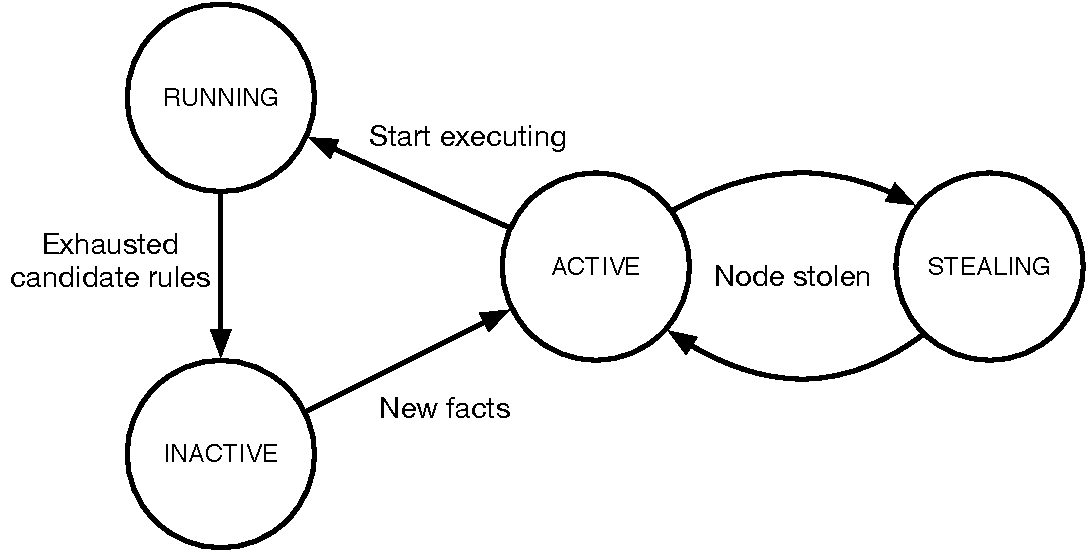
\includegraphics[width=0.55\textwidth]{figures/local/node_state.pdf}
   \mycap{The node state machine.}
   \label{fig:local:node_states}
\end{figure}

As shown in Fig.~\ref{fig:local:node_overview}, each node contains the
following attributes:

\begin{itemize}
   \item \emph{State}: the node state flag.
   \item \emph{State Lock}: a lock that protects the following node attributes:
      \emph{State}, \emph{Owner} and \emph{Incoming Fact Buffer}.
   \item \emph{DB Lock}: a lock that protects \emph{Linear DB},
      \emph{Persistent DB} and \emph{Rule Engine}. The lock is held when the
      node is applying rules or when incoming facts from other nodes need to be added to the database data
      structures.
   \item \emph{Rule Engine}: a data structure that detects which rules are
      candidates and should be derived. The data structure is fully explained
      in Section~\ref{section:local:rule_engine}.
   \item \emph{Owner}: a pointer to the thread responsible for executing this
      node.
   \item \emph{Incoming Fact Buffer}: a data structure that holds incoming facts that
      could not be added to the database data structures since the node is
      currently applying rules.
   \item \emph{Linear DB}: the database of linear facts as a set of
      structures for storing linear facts for each linear predicate.
   \item \emph{Persistent DB}: the database of persistent facts.
\end{itemize}

\begin{figure*}[t]
\centering
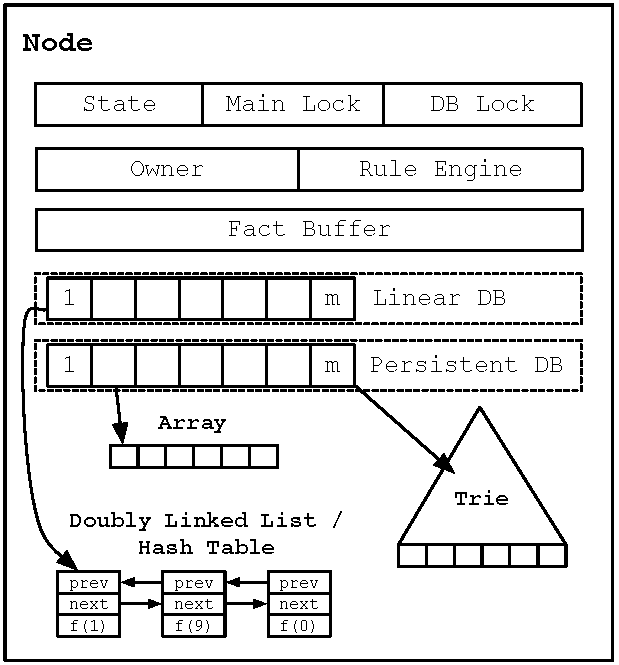
\includegraphics[width=0.5\textwidth]{figures/local/node.pdf}
\mycap{Layout of the node data structure.}
\label{fig:local:node_overview}
\end{figure*}

The database of facts must be implemented efficiently because during matching of
rules we need to restrict the facts using \emph{join constraints}, which fix
arguments of predicates to instantiated values. A database fact is made up of 2
pointers (\code{prev} and \code{next}) and a variable number of arguments. The
first (node) argument of each fact is not stored in memory since facts are
already indexed by node. Additionally, facts are indexed by predicate and use
one of the following data structures:

\begin{itemize}

\item \emph{Trie Data Structures} are used to store persistent facts. Tries are
   trees where facts are indexed by common prefix arguments. The \code{prev} and
   \code{next} pointers are used to navigate through all the facts stored in the
   trie.

\item \emph{Array Data Structures} are used to store persistent facts that are
   used in the LHS of rules that do not require matching (e.g., no join
   constraints) and exist only as initial facts. Facts stored in this data
   structure do not have the \code{prev} and \code{next} pointers because they
   are already chained by being part of a contiguous memory area. The compiler
   performs static analysis of the program's rules in order to choose between
   trie and array data structures for a particular persistent predicate.

\item \emph{Doubly Linked List Data Structures} are used to store linear facts.
   We use a doubly linked list because adding and removing facts are efficient
   operations.  The \code{prev} and \code{next} pointers are used to chain the
   facts of the linked list.

\item \emph{Hash Tree Data Structures} are used to improve lookup when linked
   lists are too long and when we need to do search filtered by a fixed
   argument. The virtual machine decides which arguments are best to be indexed
   (see Section~\ref{sec:implementation:indexing}) and then uses a hash table
   indexed by the appropriate argument. If we need to go through all the facts,
   we just iterate through all the facts in the table. Facts are hashed by using
   the indexed argument and each item in the table corresponds to a value that
   contains a list of facts with such argument. When a hash bucket has too
   many values, then the bucket is expanded from a linked list into another hash
   table, creating a hash tree~\cite{Bagwell01idealhash}.

\end{itemize}

Figure~\ref{fig:implementation:hash_table} shows an example for a hash table
data structure for a \code{p(node, int, int)} predicate with 5 linear facts
indexed by the third argument. Note that for each bucket, facts are indexed by
either a list or another hash table, recursively.

\begin{figure}[ht]
   \centering
   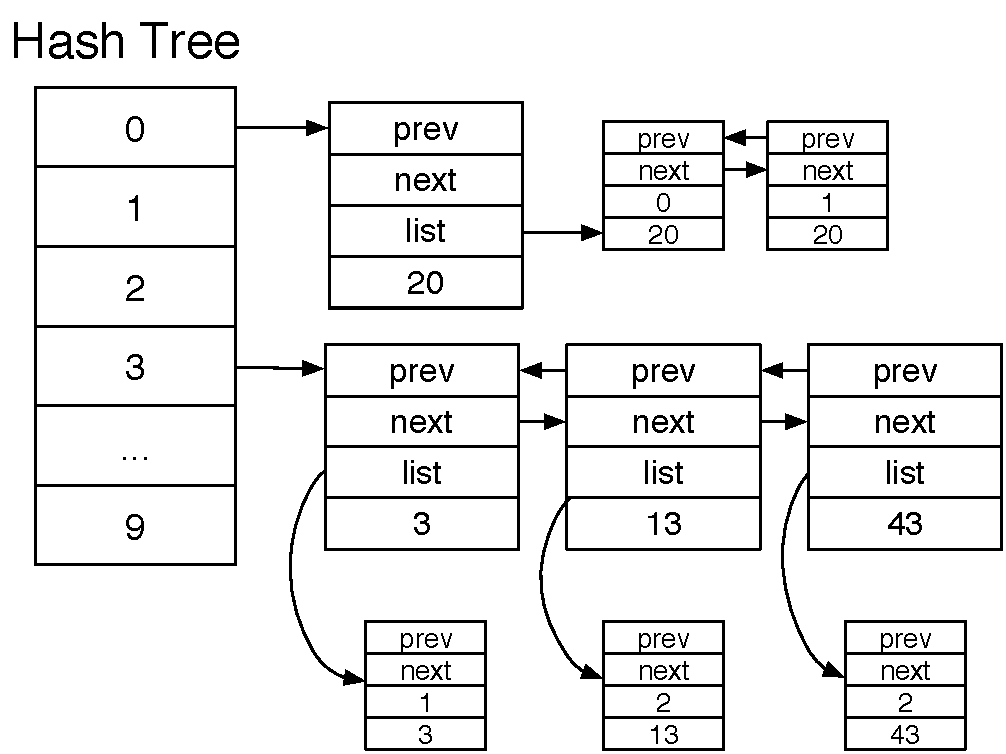
\includegraphics[width=0.6\textwidth]{figures/implementation/hash_table.pdf}

   \mycap{Hash tree data structure for a \code{p(node, int, int)} predicate
   containing the following facts: \code{p(@1, 0, 20)}, \code{p(@1, 1, 20)},
   \code{p(@1, 1, 3)}, \code{p(@1, 2, 13)}, and \code{p(@1, 2, 43)}. Facts are
   indexed by computing $arg_2\mod{}10$ where $arg_2$ is the third argument of
   the fact. The node argument is not stored.}

   \label{fig:implementation:hash_table}
\end{figure}

%%%%%%%%%%%%%%%%%%%%%%%%%%%%%%%%%%%%%%%%%%%%%%%%%%%%%%%%%%%%%%%%%%%%%%

\subsection{Indexing Engine}\label{sec:implementation:indexing}

During rule derivation, facts to be searched and filtered to match the rule
constraints. One of the most common constraints is to ensure that some arguments
of facts are equal to an arbitrary value. In order to avoid iterating over all
the facts in such cases, the VM employs a dynamic mechanism that decides,
heuristically, which argument may be optimal to index. When a predicate is
indexed, it will use a hash tree data structure instead of doubly linked list for
faster lookup. The indexing algorithm is executed along with normal computation
and empirically tries to assess the argument of each predicate that more equally
spreads the database across the values of the argument. 

The indexing algorithm is performed in three main steps and executes only in one
thread of the VM, along with normal computation. First, the algorithm gathers
lookup statistics by keeping a counter for each predicate's argument. Every time
a fact search is performed where arguments are fixed to a value, the counter of
such arguments is incremented. This phase is performed during rule execution for
the first 100 nodes (or 1\% of the nodes of the graph, when there are more than
100000 nodes) that are executed by the thread running the indexing algorithm.

The second step of the algorithm selects the candidate arguments of each
predicate. If a search for a predicate required no fixed arguments, then the
predicate will be not indexed. If only one argument was fixed, then that
argument immediately becomes the indexing argument. Otherwise, the top 2
arguments are selected for the third phase, where \emph{entropy statistics} are
collected dynamically.

During the third phase, each candidate argument has an entropy score. Before a
node transitions to the \textbf{running} state, the facts of the predicate are
used in the following formula applied for the two arguments:

\[
Entropy(F, A) = - \sum_{v \in values(F, A)} \frac{count(F, A = v)}{total(F)} \log_2 \frac{count(F, A = v)}{total(F)}
\]

\noindent where $A$ is the target argument, $F$ is the set of linear facts for
the target predicate, $values(F, A)$ is set of values of the argument $A$,
$count(F, A = v)$ counts the number of linear facts where argument $A$ is equal
to $v$ and $total(F)$ counts the number of linear facts in $F$.  The entropy
value is a good metric because it tells us how much information is needed to
describe an argument. If more information is needed, then that must be the best
argument to index.

For each argument, the $Entropy(A, F)$ value is then multiplied by the number of
times it has been used for lookup. The argument with the best score is selected
and then a global variable called \code{indexing\_epoch} is updated to
\textbf{completed}. When nodes are executed and the global
\code{indexing\_epoch} variable has changed to \textbf{completed}, the node data
structures are rebuilt by transforming doubly linked lists into hash tree data
structures. Note that the transformation is only done if the linked list has a
large number of facts (at least eight).

The VM dynamically augments hash trees if necessary. When a hash tree bucket
has too many elements, a child hash tree node is created.  On the other hand, if
the number of elements in the hash node gets too small, then the hash node is
removed and replaced with a doubly linked list.

We have seen good results with this scheme. The overhead of dynamic indexing is
negligible since the whole algorithm is performed only once.  The programmer can
also add indexes statically, if needed, using the directive \code{index
pred/arg}, where \code{pred} is the argument name and \code{arg} is the argument
number to index.

